% The generic preamble
\documentclass[10pt,letterpaper,fleqn,titlepage]{report}

% Define packages to use
\usepackage{natbib}
\usepackage[dvips]{graphicx,color}
\usepackage{amsmath,amssymb}
\usepackage{bm}
\usepackage{caption}
\usepackage{xr}
\usepackage{ifthen}
\usepackage[dvipdfm,colorlinks,linkcolor=blue,citecolor=blue,urlcolor=blue]{hyperref}
\usepackage{fancybox}
\usepackage{textcomp}
\usepackage{fancyhdr}
\usepackage{titlesec}
\usepackage{multirow}
\usepackage{alltt}
\usepackage{svn}
\usepackage{longtable}

\titleformat{\chapter}[frame]
  {\normalfont}
  {\filright\slshape\Huge\enspace\thechapter\enspace}
  {8pt}
  {\normalfont\Huge\filcenter\slshape\sffamily} 

\titleformat{\section}[hang]
  {\normalfont}
  {\filright\sffamily\bfseries\Large\thesection}
  {5pt}
  {\normalfont\Large\filright\sffamily\bfseries}[\vspace{2pt}\titlerule]

\titleformat{\subsection}[hang]
  {\normalfont}
  {\filright\slshape\sffamily\large\thesubsection}
  {5pt}
  {\normalfont\large\filright\slshape\sffamily} 
  
% Redefine default page
\setlength{\textheight}{9.0in}  % 1" above and below
\setlength{\textwidth}{6.75in}   % 0.5" left and right
\setlength{\oddsidemargin}{-0.25in}
\setlength{\topmargin}{0.0pt}
\setlength{\headsep}{16.0pt}

% Redefine default paragraph
\setlength{\parindent}{0pt}
\setlength{\parskip}{1.5ex plus 0.5ex minus 0.2ex}

% Define caption width and default fonts
\setlength{\captionmargin}{0.5in}
\renewcommand{\captionfont}{\sffamily}
\renewcommand{\captionlabelfont}{\bfseries\sffamily}

% Defined commands
\newcommand{\superscript}[1]{\ensuremath{^\textrm{#1}}}
\newcommand{\subscript}[1]{\ensuremath{_\textrm{#1}}}
\newcommand{\invcm}{\textrm{cm\superscript{-1}}}
\newcommand{\micron}{\ensuremath{\mu\textrm{m}}}
\newcommand{\textbfm}[1]{\boldmath\ensuremath{#1}\unboldmath}
\newcommand{\water}{\textrm{H\subscript{2}O}}
\newcommand{\carbondioxide}{\textrm{CO\subscript{2}}}
\newcommand{\ozone}{\textrm{O\subscript{3}}}
\newcommand{\methane}{\textrm{CH\subscript{4}}}
\newcommand{\nitrousoxide}{\textrm{N\subscript{2}O}}
\newcommand{\carbonmonoxide}{\textrm{CO}}

% Define how equations are numbered
\numberwithin{equation}{chapter}
\numberwithin{figure}{chapter}
\numberwithin{table}{chapter}

% Space/nudging commands
\newcommand{\rb}[1]{\raisebox{1.5ex}[0pt]{#1}}

%Redefine the enumerate environment to decrease the item spacing.
\let\oldenumerate=\enumerate
\let\endoldenumerate=\endenumerate
\renewenvironment{enumerate}{%
  \begin{oldenumerate}%
    \setlength{\itemsep}{0ex}%
  }%
  {%
  \end{oldenumerate}%
  }

% Define a command for title page author email footnote
\newcommand{\email}[1]
{%
  \renewcommand{\thefootnote}{\alph{footnote}}%
  \footnote{#1}
  \renewcommand{\thefootnote}{\arabic{footnote}}
}

% Redefine the maketitle macro
\makeatletter
\renewcommand{\maketitle}
{%
  \thispagestyle{empty}
  \vspace*{1in}
  \begin{center}%
     \sffamily
     {\huge\bfseries Joint Center for Satellite Data Assimilation\par}%
  \end{center}
  \begin{flushleft}%
     \sffamily
     \vspace*{0.5in}
     {\Large\bfseries CRTM: \@title\par}%
     \medskip
     {\large\@author\par}%
     \medskip
     {\large\@date\par}%
     \bigskip\hrule\vspace*{2pc}%
  \end{flushleft}%
  \newpage
  \setcounter{footnote}{0}
}
\makeatother


% Define a command for a DRAFT watermark
\usepackage{eso-pic}
\newcommand{\draftwatermark}
{
  \AddToShipoutPicture{%
    \definecolor{lightgray}{gray}{.85}
    \setlength{\unitlength}{1in}
    \put(2.5,3.5){%
      \rotatebox{45}{%
        \resizebox{4in}{1in}{%
          \textsf{\textcolor{lightgray}{DRAFT}}
        }
      }
    }
  }
}


% Generic fixed font command
\newcommand{\f}[1]{\texttt{#1}}

% Title info
\title{Subversion Repository Guide}
\author{Paul van Delst\email{paul.vandelst@noaa.gov}\\JCSDA/EMC/SAIC}
\date{September, 2008}


%-------------------------------------------------------------------------------
%                            Ze document begins...
%-------------------------------------------------------------------------------
\begin{document}
\maketitle

\hyperbaseurl{https://svn.ncep.noaa.gov/emc/}

\draftwatermark

% The tables of content
%======================
\setcounter{page}{1}
\pagenumbering{roman}
  \tableofcontents\newpage
  \listoffigures\newpage
  \listoftables\newpage
\pagenumbering{arabic}
\setcounter{page}{1}


\chapter{Introduction}
%=====================
This document describes the CRTM subversion repository and how to set up your environment to allow you to build the CRTM library, and any associated programs, directly in your working copy. It is assumed the user is familiar with Subversion.

The CRTM is one of many projects in main EMC repository on the subversion server \texttt{svn.ncep.noaa.gov}. The location of the CRTM project repository is \f{https://svn.ncep.noaa.gov/emc/crtm}. Note that, as of September 2008, the EMC repository is still behind the NCEP firewalls and access is available only to users on the NCEP network, or via a VPN connection into the NCEP network.


\chapter{Repository Organisation}
%================================
If you access the repository via your browser, you should see something like figure \ref{fig:main_repository}, where the repository is organised into the usual \f{trunk}, \f{branches}, and \f{tags} subdirectories.
\begin{figure}[htb]
  \centering
  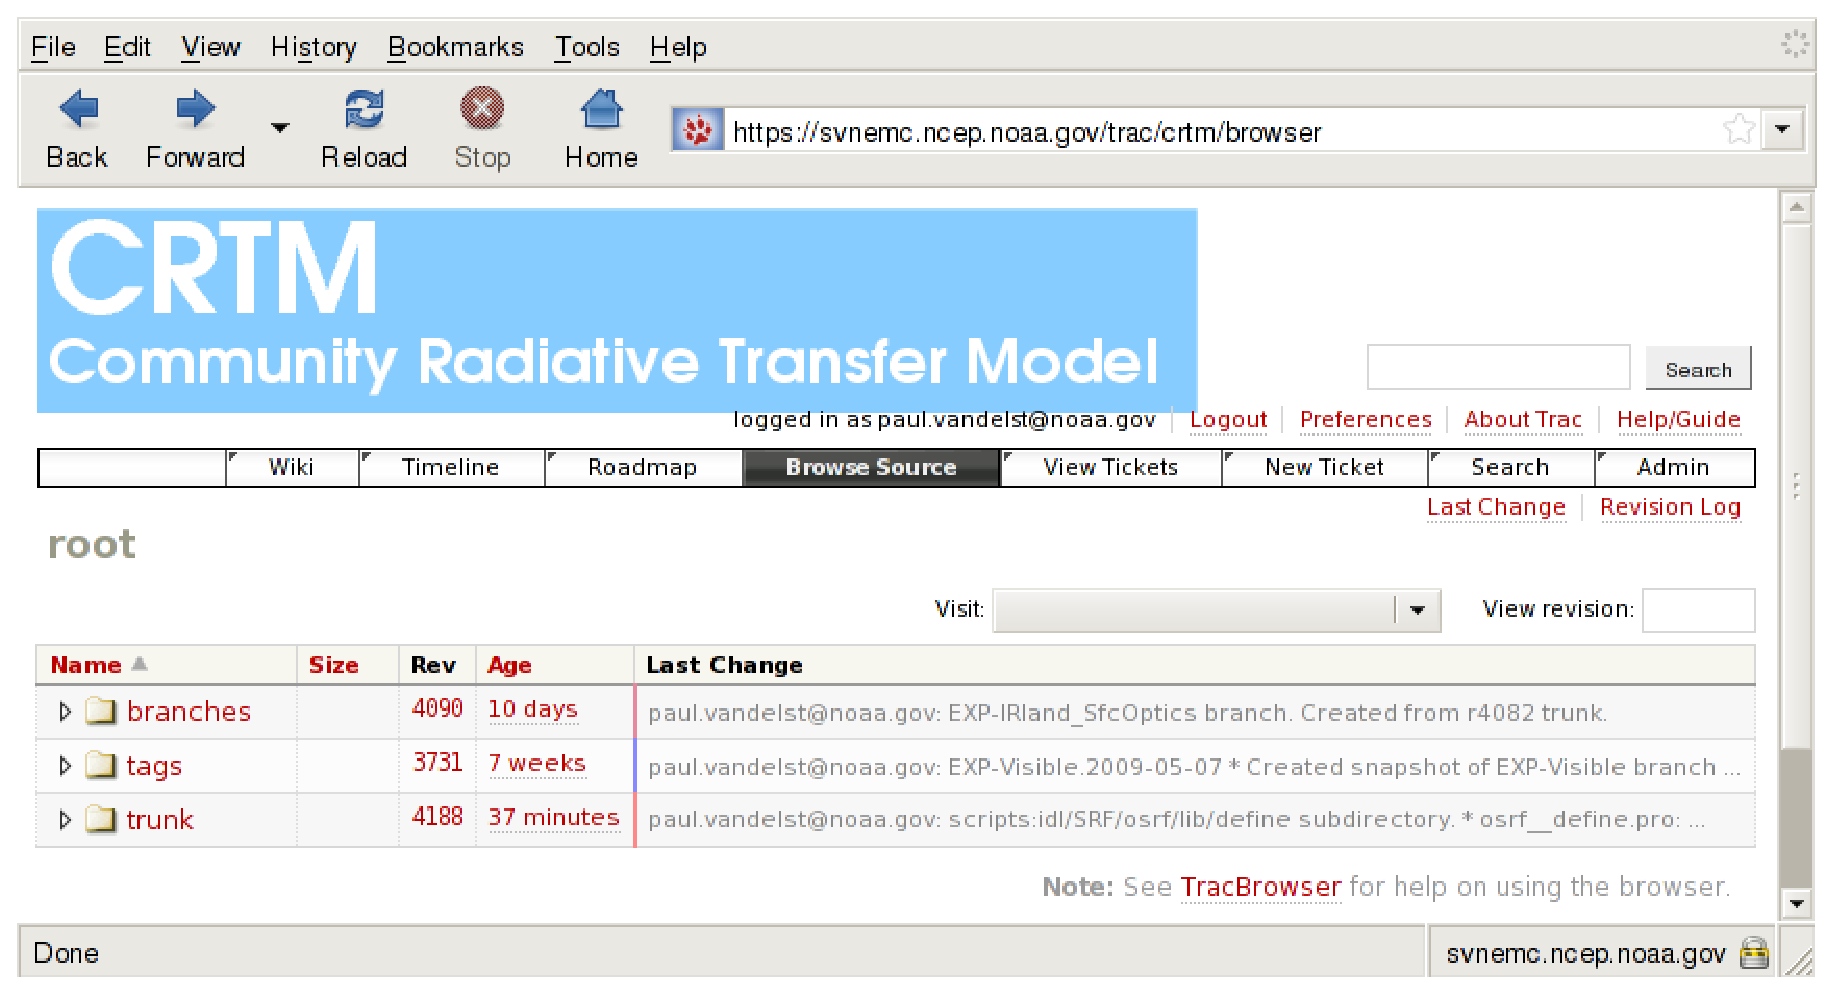
\includegraphics[scale=0.5]{graphics/main_repository.eps}
  \caption{The root of the CRTM repository organised into the typical \f{trunk}, \f{branches}, and \f{tags} subdirectories.}
  \label{fig:main_repository}
\end{figure}

\section{\f{trunk} subdirectory}
%------------------------------------
Mainline development of the CRTM is done in the trunk. Navigating the \href{crtm/trunk}{\f{trunk}} link of the web page shown in figure \ref{fig:main_repository}, displays the various categories of the CRTM repository as shown in figure \ref{fig:trunk_repository}. 
\begin{figure}[htb]
  \centering
  \includegraphics[scale=0.5]{graphics/trunk_repository.eps}
  \caption{The trunk of the CRTM repository, showing the various categories.}
  \label{fig:trunk_repository}
\end{figure}
A short description of the trunk subdirectories are shown in table \ref{tab:trunk_category_description}
\begin{table}[htb]
  \centering
  \begin{tabular}{p{2cm} p{12cm}}
    \hline
    \sffamily\textbf{Category} & \sffamily\textbf{Description} \\
    \hline\hline
    \f{doc}       & CRTM documentation\\
    \f{externals} & Library of third party software used in the CRTM and/or support software\\
    \f{fix}       & Coefficient datafiles used by the CRTM.\\
    \f{scripts}   & Hierarchy of script software, for various languages, used in CRTM build, testing, visualisation, etc.\\
    \f{src}       & Main CRTM Fortran95 source code directory. Contains the core CRTM modules as well as support software.\\
    \f{test}      & CRTM testing. Contains all the tests (unit, component) used to validate the CRTM.\\
    \f{web}       & The CRTM webpage source.\\
    \hline
  \end{tabular}
  \caption{Description of the contents of the CRTM repository trunk categories.}
  \label{tab:trunk_category_description}
\end{table}

As indicated, the \f{src} subdirectory is the one that contains the actual CRTM source code. This and the \f{fix}
directory, which contains all of the spectral, transmittance, aerosol, cloud, and surface emissivity coefficient datafiles, are the two main parts of the CRTM repository.


\section{\f{branches} subdirectory}
%---------------------------------------
Development independent of the main CRTM trunk is done in the branches subdirectory. Currently, the CRTM contains only \f{src} category branches and, of those, there are two types:
\begin{enumerate}
  \item Experimental developmental branches where wholescale changes to the CRTM may result in instability. The naming convention is \f{EXP-}\textit{desc} where \textit{desc} is a short description of the experiment. For example, a branch named \f{EXP-DISORT} has been created to implement the DISORT radiative transfer solver in the CRTM for validation. 
  \item Code release branches where the code is tested and ``tweaked'' prior to a release. The naming convention here is \f{RB-}\textit{rel} where \textit{rel} is the planned release version number. An example would be the v1.2 release branch, \f{RB-1.2}.
\end{enumerate}
The current state of the CRTM \f{branches/src} subdirectory is shown in figure \ref{fig:branches_src_repository}
\begin{figure}[htb]
  \centering
  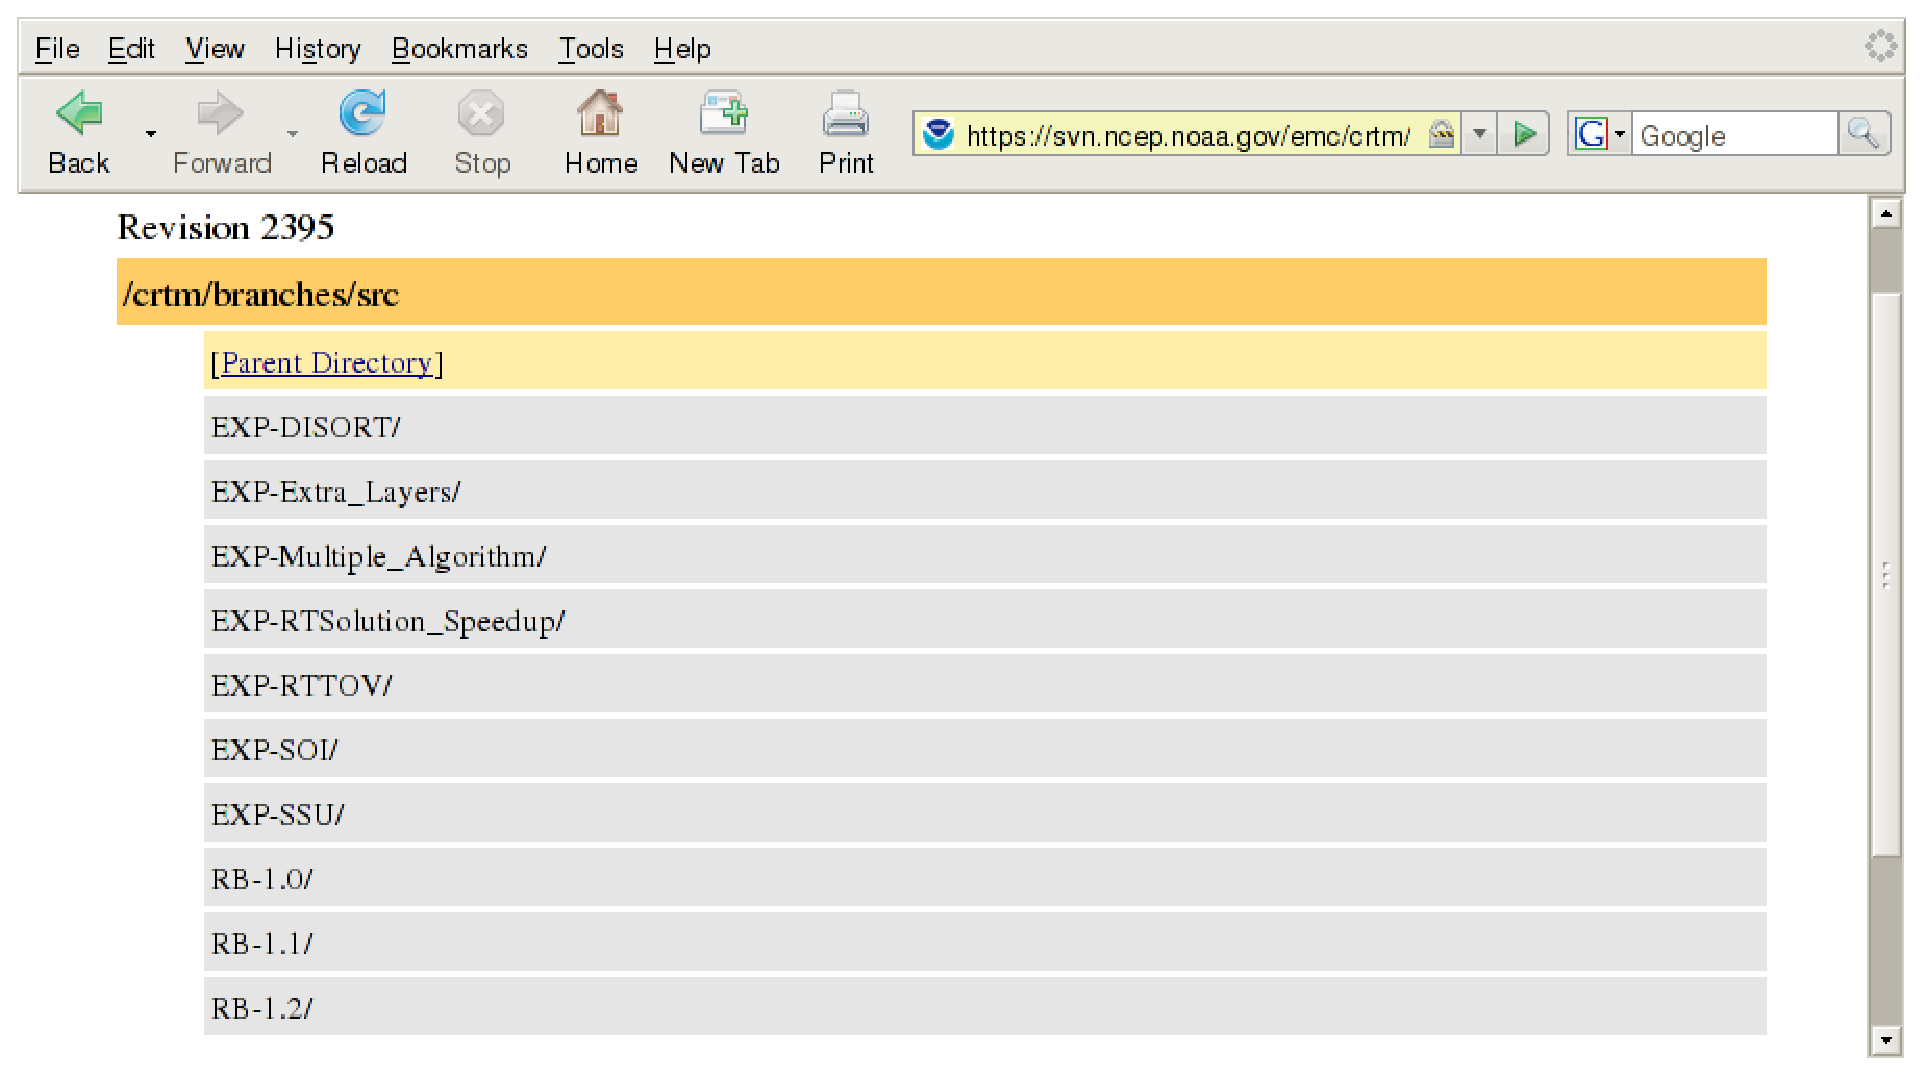
\includegraphics[scale=0.5]{graphics/branches_src_repository.eps}
  \caption{Snapshot of the \f{branches/src} subdirectory of the CRTM repository, showing the current branches.}
  \label{fig:branches_src_repository}
\end{figure}

\section{\f{tags} subdirectory}
%-----------------------------------
If a snapshot of development is wanted, or if development has been completed on a trunk or branch revision, a copy is made and placed in the \f{tags} subdirectory. There are three tag naming conventions in current use:
\begin{enumerate}
  \item For official software releases, \f{REL-}\textit{rel}; where \textit{rel} is the software relase number. For example, the first official CRTM release has the tag \f{REL-1.1}.
  \item For pre-release snapshots, \f{REL-}\textit{rel}\f{\_}\textit{stage}\f{.rev}\textit{RN}\f{.}\textit{YYYY-MM-DD}; where \textit{stage} is the release stage, typically \f{alpha} or \f{beta}; \textit{RN} is the repository revision number from which the tag was created; and \textit{YYYY-MM-DD} is the date on which the tag was created. An example of this is \f{REL-1.1\_beta.rev1855.2008-02-25}.
  \item For experimental branch snapshots, \f{EXP-}\textit{desc}\f{.rev}\textit{RN}\f{.}\textit{YYYY-MM-DD}; where \textit{desc} is a short description of the experimental branch. An example of this is \f{EXP-Extra\_Layers.rev1738.2008-02-12}.
\end{enumerate}
Some examples of the current tags in the CRTM \f{tags/src} subdirectory are shown in figure \ref{fig:tags_src_repository}. Note that there is no development in a tag directory - it is strictly a snapshot of a trunk or branch revision.

\begin{figure}[htb]
  \centering
  \includegraphics[scale=0.5]{graphics/tags_src_repository.eps}
  \caption{Snapshot of the \f{tags/src} subdirectory of the CRTM repository, showing some current tags.}
  \label{fig:tags_src_repository}
\end{figure}


\chapter{Build Conventions}
%==========================
This sections details the environment setup to enable the CRTM library, or any support software, to be compiled in a user's working copy. For the purposes of explanation we will assume that the entire CRTM trunk working copy has been checked out using something like the following commands,
\begin{ttfamily}
  \begin{verbatim}
     cd $HOME/CRTM
     svn checkout https://svn.ncep.noaa.gov/emc/crtm/trunk trunk\end{verbatim}
\end{ttfamily}
where a user's home directory is referred to by the environment variable \f{\$HOME}, and the root directory of a user's working copy of the CRTM is \f{\$HOME/CRTM} and reflects the same directory structure as the repository.

Additionally, it is assumed there exists a user directory, \f{\$HOME/bin}, which is defined in a user's \f{\$PATH}. Compiled executables and scripts will be placed in this directory.


\section{Macro Definitions}
%--------------------------
All of the makefiles in the CRTM repository use environment variables as required to locate the particular category subdirectories described in table \ref{tab:trunk_category_description}. The environment variable names, along with example definitions for a working copy are shown in table

\begin{table}[htb]
  \centering
  \begin{tabular}{p{4.5cm} p{9.5cm}}
    \hline
    \sffamily\textbf{Environment Variable Name} & \sffamily\textbf{Example Definition} \\
    \hline\hline
                                & \f{\$HOME/CRTM/trunk/src}, or \\
    \rb{\f{CRTM\_SOURCE\_ROOT}} & \f{\$HOME/CRTM/branches/src/RB-1.2}\\
    \f{CRTM\_FIXFILE\_ROOT}     & \f{\$HOME/CRTM/trunk/fix} \\
    \f{CRTM\_TEST\_ROOT}        & \f{\$HOME/CRTM/trunk/test} \\
    \f{CRTM\_SCRIPTS\_ROOT}     & \f{\$HOME/CRTM/trunk/scripts} \\
    \f{CRTM\_EXTERNALS\_ROOT}   & \f{\$HOME/CRTM/trunk/externals} \\
    \f{CRTM\_DOC\_ROOT}         & \f{\$HOME/CRTM/trunk/doc} \\
    \hline
  \end{tabular}
  \caption{Environment variables used by CRTM makefiles.}
  \label{tab:macro_description}
\end{table}

Ideally, the environment variables of table \ref{tab:macro_description} should be defined in a user's environment definition file to ensure they will be defined in any shell invocation.

For now, just note the multiple examples for the \f{CRTM\_SOURCE\_ROOT} macro. The reason for this will be explained later (see section \ref{sec:crtm_build}).


\section{Install of script files}
%--------------------------------
The simplest way to build a library is to have all the source code in a single directory. The CRTM source code modules in the \f{src} directory, however, are organised into separate subdirectory hierarchies according to their application. It is expected that this organisational structure will change over time. Rather than create makefiles that need to know what the directory structure is to find all the various source files, a shell script (\f{linkfiles}) is used to link all the necessary files into the CRTM library build subdirectory, \f{src/Build}.

So, the second step in setting up the CRTM build environment is to install the necessary scripts. The current method for doing this is through unsophisticated use of makefiles. The sequence of commands for the script install are,
\begin{ttfamily}
  \begin{verbatim}
     cd $CRTM_SCRIPTS_ROOT/shell/Utility
     make install\end{verbatim}
\end{ttfamily}
This installs all the scripts currently used in the CRTM build process. Note there is also an uninstall target that removes all the scripts from a user's local \f{bin} directory.

\section{Master Make Include Files}
%----------------------------------
\label{sec:make_includes}
All of the makefiles in the CRTM repository use three standard include files: \f{make.macros}, \f{make.common\_targets} and \f{make.rules}. These files reside in the \f{CRTM\_SOURCE\_ROOT} subdirectory and their function is described in table \ref{tab:make_includes}.

\begin{table}[htb]
  \centering
  \begin{tabular}{p{4.5cm} p{9.5cm}}
    \hline
    \sffamily\textbf{Include File Name} & \sffamily\textbf{Description} \\
    \hline\hline
    \f{make.macros}          & Defines macros for all the compiler and linker flags for the supported compiler/platform combinations, as well as commonly used operating system commands and utilities, e.g. \f{cp}, \f{rm}, \f{ar}, etc. \\
    \f{make.common\_targets} & Defines the common targets used in builds, e.g. \f{all}, \f{install}, \f{clean}, etc. \\
    \f{make.rules}           & Defines the suffix rules for compiling Fortran source code. \\
    \hline
  \end{tabular}
  \caption{Include files used by CRTM makefiles.}
  \label{tab:make_includes}
\end{table}


\section{Building the CRTM Library}
%----------------------------------
\label{sec:crtm_build}
Having setup the environment on a system, the sequence of commands to build and install the CRTM library in a checked out working copy is,
\begin{ttfamily}
  \begin{verbatim}
     cd $CRTM_SOURCE_ROOT
     make create_links
     make
     make install\end{verbatim}
\end{ttfamily}
The first target, \f{create\_links}, searches for all the required CRTM source code starting at \f{\$CRTM\_SOURCE\_ROOT} and links it all into the \f{Build/src} subdirectory\footnote{For some systems, notably the IBM systems at NCEP, this can take several minutes. For linux desktop systems, it should only take a few seconds. A ruby version of the script does exist that is quite a bit faster.}.

The second make does the actual source code compilation and library creation.

The last target, \f{install}, moves the created CRTM library, \f{libCRTM.a}, into the \f{Build/lib} subdirectory and all of the associated \f{*.mod} module files into the \f{Build/include} subdirectory.

If you wish to build a particular branch or release (tag) of the CRTM library, all you need to do is redefine the \f{CRTM\_SOURCE\_ROOT} environment variable to your working copy location for that branch or release. The redefinition can be system-wide (e.g. if you're working solely on a release branch in preparation for the release) or for a single shell session (e.g. if you're building an older or experimental version alongside the current release).

If the build is a final one (e.g. you're not testing the CRTM), the \f{Build/lib} and \f{Build/include} subdirectories are typically copied or moved to a generic location outside of the working copy, e.g. \f{\$HOME/local/lib} and \f{\$HOME/local/include}, or \f{\$HOME/local/CRTM/lib} and \f{\$HOME/local/CRTM/include}

As mentioned in section \ref{sec:make_includes}, compiler flags for varous platforms (or in the case of linux, for various compilers) are defined in the \f{make.macros} file. Instructions on how to modify the \f{make.macros} for different compilers on a linux systems can be found in the \f{Build/README} file.

\section{Cleaning up}
%--------------------
There are three targets that tidy up after a CRTM build. Depending on your needs they clean up intermediate files to varying degrees. A description of the clean targets is shown in table \ref{tab:clean_up}.

\begin{table}[htb]
  \centering
  \begin{tabular}{p{2.5cm} p{11.5cm}}
    \hline
    \sffamily\textbf{Target Name} & \sffamily\textbf{Description} \\
    \hline\hline
    \f{clean}     & Removes all the \f{*.o}, \f{*.mod}, \f{*.a} files from the \f{Build/src} subdirectory. \\
    \f{distclean} & Same as \f{clean} but also deletes the \f{Build/lib} and \f{Build/include} subdirectories. \\
    \f{realclean} & Same as \f{distclean} but also deletes the source code symbolic links in the \f{Build/src} subdirectory.\\
    \hline
  \end{tabular}
  \caption{Cleanup targets in the CRTM library build makefiles.}
  \label{tab:clean_up}
\end{table}
If you invoke the \f{realclean} target and want to subsequently rebuild the CRTM libarry, you will have to recreate the links as detailed in section \ref{sec:crtm_build}. And, remember, creating the links can take some time on some systems.


\begin{appendix}

\end{appendix}


\end{document}

